\chapter{Evaluation}
\label{evaluation}

In this chapter, CCDetect-LSP will be evaluated based on different criteria, which combined
will provide a basis for evaluating the tool as a whole.

The most important aspect of CCDetect-LSP to evaluate is its performance in a real-time
environment. We will compare the time of the initial detection with the incremental
detection, as well as compare its performance with another incremental clone detector,
iClones~\Cite{GodeIncrementalCloneDetection}. Note that we will also distinguish between
the initial detection where parsing the entire code base is necessary, and subsequent
detections which still constructs the suffix array from scratch, but does not require
parsing the entire code base. We will call this type of detection the SACA detection,
while the detection which uses the dynamic extended suffix arrays will be called the
incremental detection. This is done to compare the dynamic extended suffix array against
building the suffix array from scratch.

This chapter will evaluate CCDetect-LSP in the following ways:

\begin{itemize}
    \item Verify correctness of clone detection with BigCloneBench
    \item Informal complexity analysis of each phase in the initial and incremental
        detection algorithms
    \item Performance benchmark of SACA detection, incremental detection and iClones
    \item Memory usage benchmark of SACA detection, incremental detection and iClones
    \item Language and IDE support
\end{itemize}



\section{Verifying clones with BigCloneBench}

In order to verify that CCDetect-LSP correctly identifies clones, we should analyze and
confirm that CCDetect-LSP finds all clones in a given code base.
BigCloneBench~\cite{BigCloneBench} is a clone detection benchmark of a set of known clones
in a Java dataset called ``IJaDataset''. The benchmark consists of the IJaDataset and a
database containing information of the clones which exist in the dataset.
BigCloneEval~\cite{BigCloneEval} is a tool which simplifies evaluation of a tool on the
BigCloneBench. BigCloneEval evaluates a tool by running the tool on the dataset, letting
the tool output all the clones the tool finds, and then matching the clones the tool found
with the clones in the database. This makes the BigCloneBench essentially a big oracle for
clone detection in a code base, which we test CCDetect-LSP against. The clones in the
database are manually verified by humans, and include type-1 to type-3 clones.

We evaluated CCDetect-LSP by running the initial detection algorithm on the dataset, and
outputting all the clones the tool found. BigCloneEval expects to get a file where each
line contains a clone pair, where a clone is specified with filename, starting and
ending line. This was simple to extract from our clone-map, where we converted our ranges
which point to the beginning and ending token, to just the line number of those tokens.

BigCloneEval reports the recall of a tool, meaning the percentage of found clones.
Therefore, we did not make sure that our conversion to the format BigCloneEval expects
gave the minimum number of clone pairs. For example, for a clone pair of clones $A$ and
$B$, we output both that $A$ is a clone of $B$ and that $B$ is a clone of $A$, which is
superfluous. This would lead to a bad precision, but does not affect the recall in the
report which BigCloneEval outputs.

For CCDetect-LSP, we used mostly the default parameters of BigCloneEval, but we increased
the minimum clone size to $100$ and set the minimum similarity threshold to be $100\%$,
since we are only evaluating CCDetect-LSP for type-1 and type-2 clone recall. Setting the
minimum similarity threshold also drastically reduces the time an evaluation takes, as we
skip evaluating detection of type-3 clones. The default token threshold was set to $100$
instead of $50$, as the evaluation time alsos increases drastically as the number of
clones to match in the database and the number of clones reported by CCDetect-LSP
increases.

For the type-2 detection, we set the following AST nodes to be normalized:

\begin{lstlisting}
    blind_nodes = [
        "name",
        "identifier",
        "string_literal",
        "decimal_integer_literal",
        "decimal_floating_point_literal",
        "type_identifier",
    ]
\end{lstlisting}

These nodes were normalized because it correlates with our definition of a type-2 clone.

Appendix \ref{bcblog} shows the command which runs BigCloneEval, and the beginning of the
report generated when CCDetect-LSP is evaluated. The report shows that CCDetect-LSP has a
${\sim}99.98\%$ recall for type-1 clones and a ${\sim}89.40\%$ recall for type-2 clones.
CCDetect-LSP is clearly capable of detecting type-1 clones. As for the missing type-1
clones, while it is not so simple to determine which clones were not detected, it is
possible that these clones are not reported because of inconsistencies in the database.
The report also shows that CCDetect-LSP manages to detect almost all type-2 clones. This
will be discussed further in \cref{discussion}.

\section{Time complexity of detection}

In this section we will conduct an informal analysis of the running time of each phase of
the initial, SACA and incremental detection to argue that the average runtime complexity
of the incremental detection is lower than the initial detection. In each phase we will
argue the run time in terms of Big O notation. Some claims will be substantiated in the
next section where we look at concrete code bases and their properties.

First, we will define some notation for this analysis. We are analyzing a code base of
size $n$, where $n$ is the number of characters in the code base. The fingerprint of the
code base is of size $f$, where $f$ is the number of symbols in the full fingerprint and
$f \ll n$. The alphabet of the fingerprint has a size of $\sigma$. In the incremental
detection, $E$ is an edit, consisting of $e$ characters. We will also use
$\vert\text{clones}\vert$, $\vert\text{documents}\vert$, $\vert\text{edits}\vert$ when
discussing the number of clones, documents and edits.

The initial detection runs in $O(n)$ time. The bottleneck of the initial detection is
reading and parsing all the content in each file. Tree-sitter generates Generalized LR
(GLR) parsers~\cite{GLR}, which in the worst-case have a $O(n^3)$ running time, but $O(n)$
for any deterministic grammar. As programming languages generally have deterministic
grammars, we will assume that the running time of parsing with Tree-sitter takes $O(n)$
time. After the initial parsing, the SACA detection runs in $O(f)$ time. The running time
is $O(f)$ because the suffix array construction is performed for every update, which takes
linear time in the size of the input, which is the fingerprint. The extraction of clones
from the LCP array also runs in $O(f)$ as it is a single scan over the LCP array. The
final source-mapping is a bit more complicated, taking $O(\vert\text{clones}\vert \times
\log (\vert\text{documents}\vert))$. This complexity arises from binary-searching the list
of documents to find the correct document for each clone. This is highly likely to be less
time consuming than the suffix array construction, as the number of documents and number
of clones are usually orders of magnitude lower than the size of the whole code base.
Therefore, we get a final running time of $O(f) + O(\vert\text{clones}\vert \times
\log(\vert\text{document}\vert))$, where $O(f)$ is highly likely to be the dominating
factor.

For the incremental detection, we have already parsed the code base and built the index,
dynamic extended suffix array and wavelet matrix for the code base. Afterwards, when an
edit $E$ is performed in a document $D$, the first phase is to update the document index.
We iterate over the documents to update their fingerprint ranges, which has a complexity
of $O(\vert\text{documents}\vert)$. When a document which has been edited is reached, the
new document content is incrementally parsed, queried for fragments and then the fragments
are fingerprinted. In an IDE scenario, only one file is edited in each update, so only one
document needs to be parsed in each update. In the worst-case, we have to fingerprint the
entire document, which has a complexity of $O(\vert D\vert)$. The complexity of this phase
is therefore $O(\vert\text{documents}\vert + \vert D\vert)$.

Next, extracting the edit operations which have happened to $D_f$ (fingerprint of $D$),
takes $O(\vert D_f\vert + \vert E\vert^2)$ where $\vert E\vert \leq \vert D_f\vert$. Note
that the size of the edit is calculated as the area which $E$ covers, meaning that if an
edit consists of changing a token at the beginning of the file, and a token at the end of
the file, then $\vert E\vert \approx \vert D_f\vert$. We get this time complexity because
Hirschberg's algorithm runs in $O(n \times m)$ where in our case, $n \approx m$. If the
size of the edit is contained in a smaller area, we apply the optimization which reduces
the size of the edit by comparing characters at the beginning and end of the string, as
discussed in \cref{dynamicdetection}. This process has a complexity of $O(\vert D_f\vert)$,
and afterwards Hirschberg's algorithm has a worst-case complexity of $O(\vert E\vert^2)$.

The worst-case complexity of dynamically updating the extended suffix array is actually
slower than a linear time SACA algorithm in the worst-case. The worst-case scenario when
inserting/deleting a character in the fingerprint is that every single suffix needs to be
reordered, meaning we reorder $O(f)$ suffixes, where each reordering takes $O(\log(f))$
time, as it requires deleting and inserting an element in the dynamic extended suffix
array. In addition, we need to call the LF function twice for each reordering, which has a
$O(\sigma + \log f \log\sigma)$ complexity. The complexity of the LF function comes from a
$rank$ call in the wavelet matrix, and an iteration over $C$ to find the number of smaller
characters. This results in a $O(f \times (\sigma + \log f \log\sigma))$ running time of
this phase, which is worse than the $O(f)$ running time of the SACA algorithm. In
addition, before the reordering when we are inserting/deleting characters in the BWT, we
use the LF function and insert/delete in the wavelet matrix and the $C$ array. The
dominating factor of these operations is again the LF function. If an edit operation
consists of inserting/deleting multiple characters, the number of LF function calls is
increased, with a complexity of $O(e \times (\sigma + \log f \log\sigma))$. We can extend
this to account for multiple edit operations as well, which increases the complexity to
$O(\vert\text{edits}\vert \times (e \times (\sigma + \log f \log\sigma)))$. Note that while
there are many factors in this time complexity, all the factors should be quite small
compared to $f$, making the complexity of reordering the suffixes the dominating factor of
this phase.

The average-case complexity of this phase is however highly likely to be faster. Salson et
al. have shown that on average, the number of reorderings required for an
insertion/deletion in a suffix array is highly correlated with the average LCP value of
the input~\cite{DynamicExtendedSuffixArraysReorderings}. Their data shows that for
multiple different types of data such as genome sequences and english text, the average
LCP value of the input is generally magnitudes lower than the input size. In our
experiments, this applies to source code as well, as code bases we have tested on have all
had an average LCP values well below $100$. See Table \ref{tab:codebases} to see the
average LCP value for different code bases. A lower number of reordered suffixes for lower
LCP values seems intuitive, as lower LCP values mean that the insertion/deletion will
affect the ordering of fewer suffixes in the input. With this information, it would be
more accurate to de-emphasize the importance of the $O(f)$ number of reordered suffixes in
our analysis, and we therefore claim that the average running time of an edit operation on
the suffix array is closer to $O(e \times (\sigma + \log f \log\sigma))$ if we account for
multiple characters being inserted or deleted as well. We extend this to account for
multiple edit operations as well, for each edit operations which was computed in the last
phase, we perform an insertion/deletion of $e$ characters. Therefore, the total complexity
of this phase on average is closer to $O(\vert\text{edits}\vert \times (e \times (\sigma +
\log f \log\sigma)))$.

Next there is the clone extraction phase. Recall that in the dynamic detection clone
extraction phase, we had stored all nodes with an LCP value above the token threshold, and
iterate over those to determine which of them are clones or not. In the worst-case, every
index in the LCP array would be above the token threshold, which would be an $O(f)$
complexity iteration. However, this is highly unlikely, since the nodes with LCP value
above the token threshold are either clones, or contained clones. The number of contained
clones is limited by the number of clones because each clone can only have a limited
amount of contained clones. Therefore, the number of LCP nodes examined should be closer
to $O(\vert\text{clones}\vert)$, which is highly likely to be less expensive than
iterating over all the LCP nodes. For each examined LCP node, we need to traverse from the
node, to its pointer node, and then to the root of the $B$ tree to determine the
fingerprint index of that LCP node. We do the same to determine the index of the matching
clone, as described in Chapter \ref{dynamicdetection}. These traversals take $O(\log f)$
time. The worst-case performance of this phase is therefore $O(f \times \log(f))$, but on
average the complexity is closer to $O(\vert\text{clones}\vert \times \log(f))$.

Finally, the source-mapping phase is easier to analyze. As we now know all the positions
of clones and their matches, building the clone-map takes $O(\vert\text{clones}\vert
\times \log(\vert\text{documents}\vert))$ time. We perform the binary-search over the
documents to get the source location for each clone index we found in the previous phase.
This is the same complexity for both the SACA and incremental detection.

With this informal analysis, we have demonstrated that in the average case, the
incremental detection should be faster than the SACA detection, as none of the phases
reach or exceed the $O(f)$ running time of the SACA detection. In the next section we will
show that the properties we have assumed for this analysis are present in multiple code
bases, and that these properties lead to a better benchmark performance for the
incremental detection.

\section{Benchmark performance}

For the performance benchmark we will benchmark the running time of CCDetect-LSP on code
bases and edits of different sizes. We will compare the performance of the incremental
detection with the SACA detection and iClones~\cite{GodeIncrementalCloneDetection}.

iClones is a tool which, similarly to CCDetect-LSP, does incremental clone detection. The
tool takes $n$ revisions of the same code base and will after the initial detection, reuse
as much information as possible to reduce the amount of work needed to analyze consecutive
revisions. The algorithm which iClones uses is based on generalized suffix trees (GST),
and the tool can detect up to type-3 clones. For a revision $i$, iClones expects to have a
file named \verb|changed| in the root folder of the revision, which contains information
on which files have changed between revision $i - 1$ and $i$. For each file which has
changed, the suffixes in the file is inserted into the GST, reusing nodes of the tree if
possible.

For the performance benchmark, the code bases are set up in the way iClones expects. For
each code base to analyze, we will store $n$ revisions of it, where each revision contains
some changes to some files. An evaluation program for CCDetect-LSP was written so that it
can process this same setup, making it simple to run both CCDetect-LSP and iClones on the
same code bases, and compare their results. Note that it was not feasible to perform
incremental parsing for such a setup, as this setup did not include a range for the
changed content inside a file. Instead, each file which is edited in each revision is
parsed from scratch. However, we believe that the cases where incremental parsing is
particularly useful, such as when repeatedly editing a large file, is not displayed in
such a setup anyway, as each revision will only edit a file once in each revision.

To create a larger sample set of code bases and edits, it is preferable to generate new
revisions of a code base programmatically. Generating new revisions of a code base means
that we copy the code base and apply a number of insertions/deletions to random files, to
simulate how a programmer would edit files when programming. Generating new revisions of
code bases is not a trivial problem, since each edit performed in a file should still give
a valid program which can be parsed. If the file cannot be parsed, Tree-sitter will not
give a proper AST for the file. Because of this, generating insertions is hard, because we
need to make sure that the location we are inserting some code is a valid location for
that code. It is easier to generate deletions first instead. Deletions are easier to
generate, as we can use Tree-sitter to determine where a fragment of size $n$ is located,
and remove that section of code in the next revision. For example in Java, we can delete
an entire method, and still know that the program will parse to a valid AST afterwards.
After we have generated for example $10$ revisions where the difference between each
revision is deletion of some number of fragments, we can then reverse the ordering of the
revisions, so that the final revision is now the first revision, and so on. This will
translate each deletion to instead be an insertion, as an insertion is simply an inversion
of a deletion. Figure \ref{fig:revisioninversion} illustrates how a test consisting of
three revisions with deletions can be inverted to create a test of insertions. With this
technique we can generate arbitrary tests consisting of either a number of insertions or
deletions in each revision.

\begin{figure}[t]
    \begin{center}
        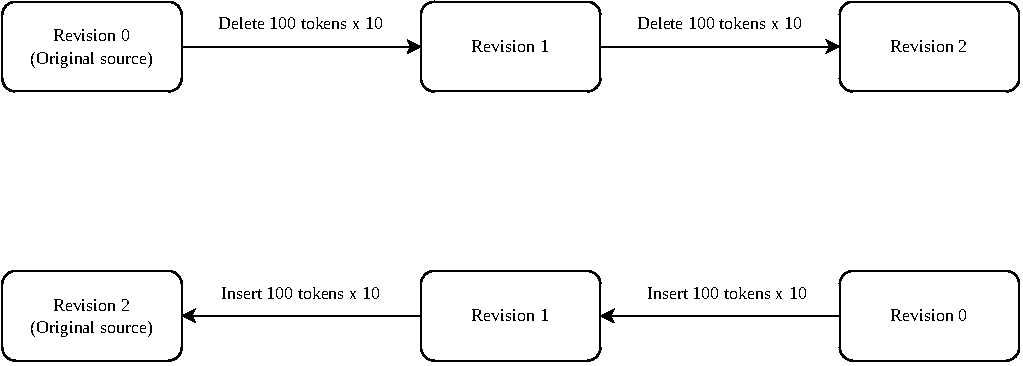
\includegraphics[width=0.95\textwidth]{figures/revisioninversion.drawio.pdf}
    \end{center}
    \caption{Reversion of an evaluation test. Delete100x10 to Insert100x10}
    \label{fig:revisioninversion}
\end{figure}

There are multiple variables we can tune when generating the tests. Primarily the three
most important factors of the tests is the size of the code base, the number of edit
operations in each revision, and the size of those edit operations.

The size of the code base will naturally affect the running time of the algorithm. We
randomly picked open-source code bases of differing sizes and differing amounts of
duplication to run the benchmark on. We selected the code bases
WorldWind\footnote{WorldWind: \url{https://github.com/NASAWorldWind/WorldWindJava}},
neo4j\footnote{neo4j: \url{https://github.com/neo4j/neo4j}}, graal\footnote{graal:
\url{https://github.com/oracle/graal}}, flink\footnote{flink:
\url{https://github.com/apache/flink}}, elasticsearch\footnote{elasticsearch:
\url{https://github.com/elastic/elasticsearch}} and
intellij-community\footnote{intellij-community:
\url{https://github.com/JetBrains/intellij-community}}. The code bases are all Java code
bases of different size, with different amounts of duplication. Table \ref{tab:codebases}
shows some properties of the code bases, including their number of lines, the number of
clones detected by CCDetect-LSP for a token threshold of $100$, the average LCP value and
the number of LCP values above $100$. An interesting aspect of the graal and flink code
bases is that they both contain ${\sim}2.2\text{MLOC}$, but graal has a higher
$\text{LCP}_\text{avg}$, which could potentially lead to a slower suffix array update,
according to our informal analysis.

\begin{table}[t]
    \begin{center}
        \begin{tabular}[c]{|l|l|l|l|l|}
            \hline
            \textbf{Code base} & \textbf{LOC} & \textbf{Clones detected} &
            $\textbf{LCP}_{\textbf{avg}}$ & $\textbf{LCP}_{\geq \textbf{100}}$ \\
            \hline
            WorldWind & 550KLOC & 1517 & 18 & 63967\\
            \hline
            neo4j & 1MLOC & 1313 & 9 & 27557\\
            \hline
            graal & 2.2MLOC & 2012 & 28 & 154452\\
            \hline
            flink & 2.3MLOC & 4729 & 13 & 155754\\
            \hline
            elasticsearch & 3.2MLOC & 9986 & 14 & 289511 \\
            \hline
            intellij-community & 5.8MLOC & 3585 & 19 & 336190 \\
            \hline
        \end{tabular}
    \end{center}
    \caption{Properties of code bases}
    \label{tab:codebases}
\end{table}

Additionally, we chose to test both an edit size of $10$ and $100$ tokens with $10$ edits
in each revision. We believe these values to be slightly larger than what is realistic for
an IDE scenario where a programmer is editing and updating the fingerprint of a single
file at a time. For a test where we are performing $10$ insertions of $100$ tokens, this
means we are inserting $1000$ tokens in a single edit, which is likely larger than any
realistic edit, but could occur in large-scale automatic refactoring operations.
Therefore, if the results shows that the algorithm can process these types of edits in
``real-time'', we believe that the algorithm can process most realistic editing scenarios.

In addition, we performed a final test on the elasticsearch code base where in each
revision, the number of edits increase. This was tested to see how CCDetect-LSP scales
when the number of edits increase. The size of these edits are not realistic for the IDE
scenario, as when the number of edits increases, thousands of tokens are being edited in a
single revision. However, this could be more realistic for the evolution scenario. Recall
that the evolution scenario is when we analyze different revisions of a code base such as
different commits in version control.

The benchmarks were run on a computer with 16GB RAM, and an Intel i7-2600K CPU with a
3.4GHz clock speed and 4 cores\footnote{Note that this CPU is quite old, and may not be
representative of today's modern CPUs}. The computer runs Manjaro Linux with kernel
version 6.1.25-1. The SACA detection, incremental detection and iClones was run with a
token threshold of $100$, and the processing time of each revision was timed using a
simple clock mechanism programmed in Java. CCDetect-LSP did not normalize any AST node
types in this evaluation, so CCDetect-LSP detects strictly type-1 clones in this
benchmark. We do not believe detection of type-2 clones would affect the performance
benchmarks signficantly. Type-3 clone detection was disabled for iClones with the
\verb|-minclone 100| parameter. Each test was run three times, and the results were
averaged. Only three runs of all tests were performed because running all the tests takes
a significant amount of time (multiple hours), and the results seem to be stable from
three runs only.



Figure \ref{fig:WorldWind}, \ref{fig:neo4j}, \ref{fig:graal}, \ref{fig:flink},
\ref{fig:elasticsearch}, \ref{fig:intellij} and \ref{fig:elasticsearch_inc} shows the
benchmark results on the different code bases. Each graph shows the running time of the
SACA detection, the incremental detection and iClones when run on a certain code base and
edit operation size. For each code base there were four tests, where two graphs consider
deletions of size $10$ or $100$ (DEL10, DEL100) and two graphs consider insertions of size
$10$ or $100$ (INS10, INS100). The running time is shown on a log scale, as the initial
detection is extremely slow compared to the subsequent detections. iClones was not able to
run on the intellij-community code base, as the memory usage exceeded 16GB, therefore only
the CCDetect-LSP algorithms is shown on those graphs. The elasticsearch code base with a
size of $3.2\text{MLOC}$ was approximately the maximum size code base iClones could run on
before the computer ran out of available memory. Note that figure
\ref{fig:elasticsearch_inc} shows the test where an increasing number of edits were
performed in each revision, the number of edits are displayed as the labels of the x-axis.

\newpage
\null
\vfill

\begin{figure}[H]
    \begin{center}
        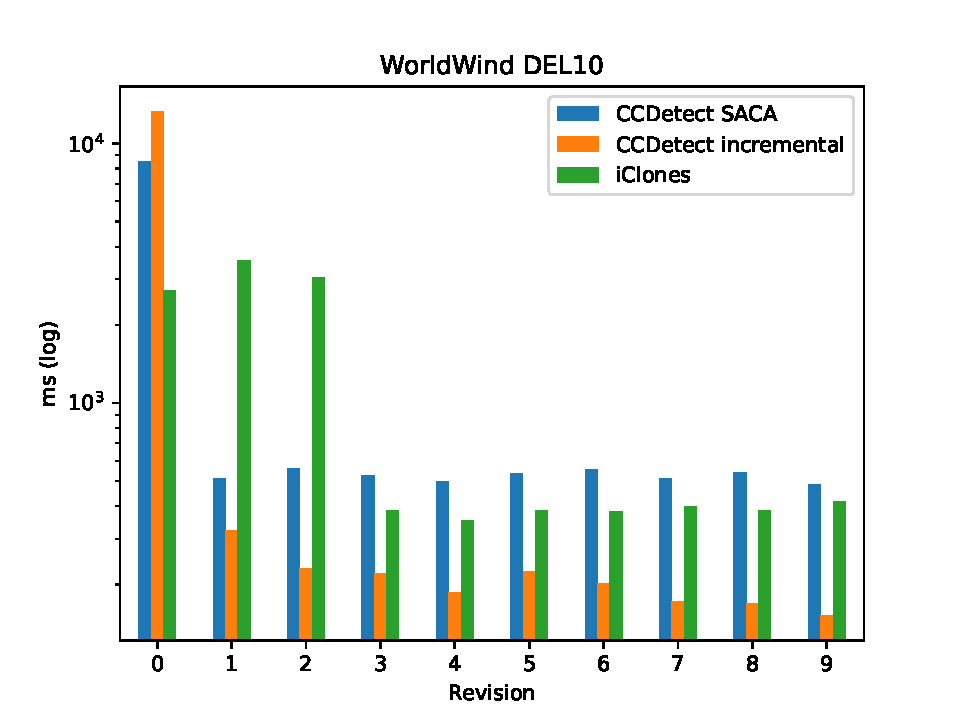
\includegraphics[width=0.49\textwidth]{figures/performancegraphs/WorldWind_DEL10.pdf}
        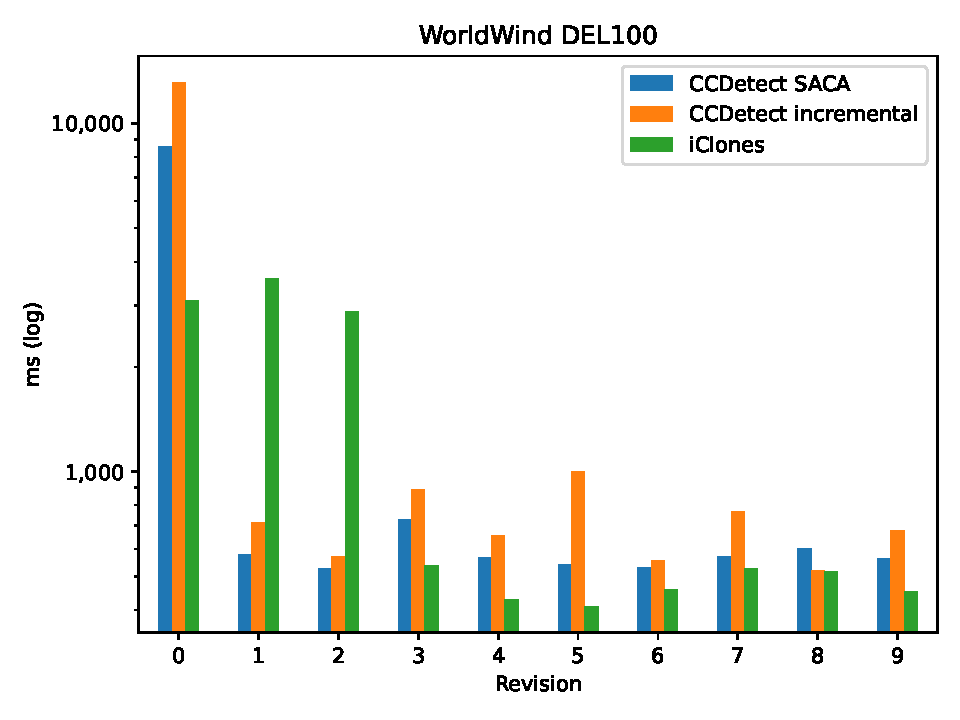
\includegraphics[width=0.49\textwidth]{figures/performancegraphs/WorldWind_DEL100.pdf}
        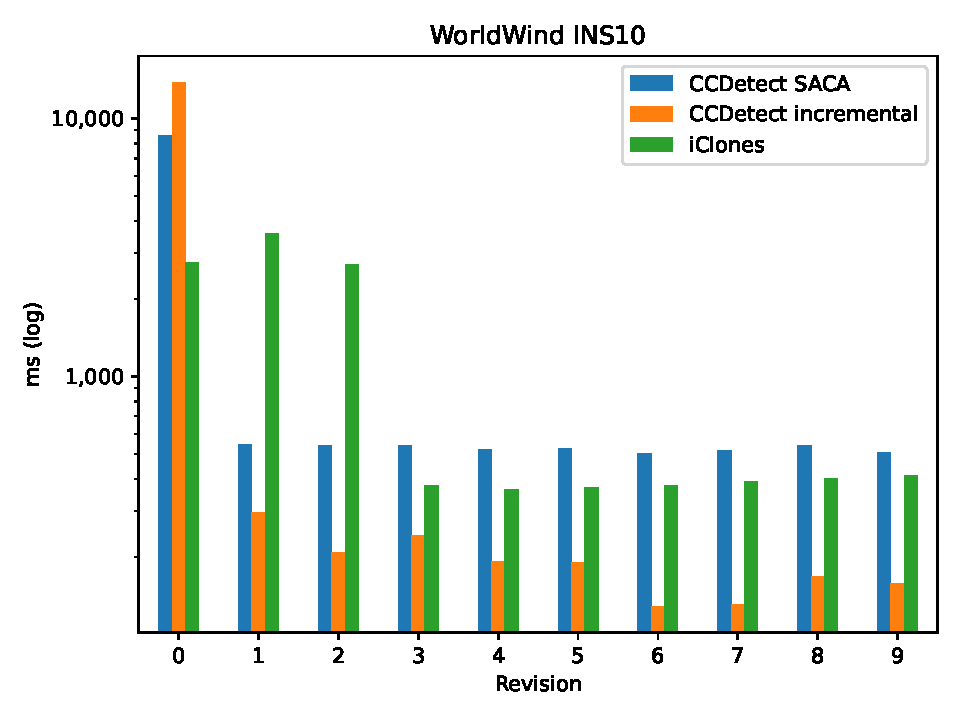
\includegraphics[width=0.49\textwidth]{figures/performancegraphs/WorldWind_INS10.pdf}
        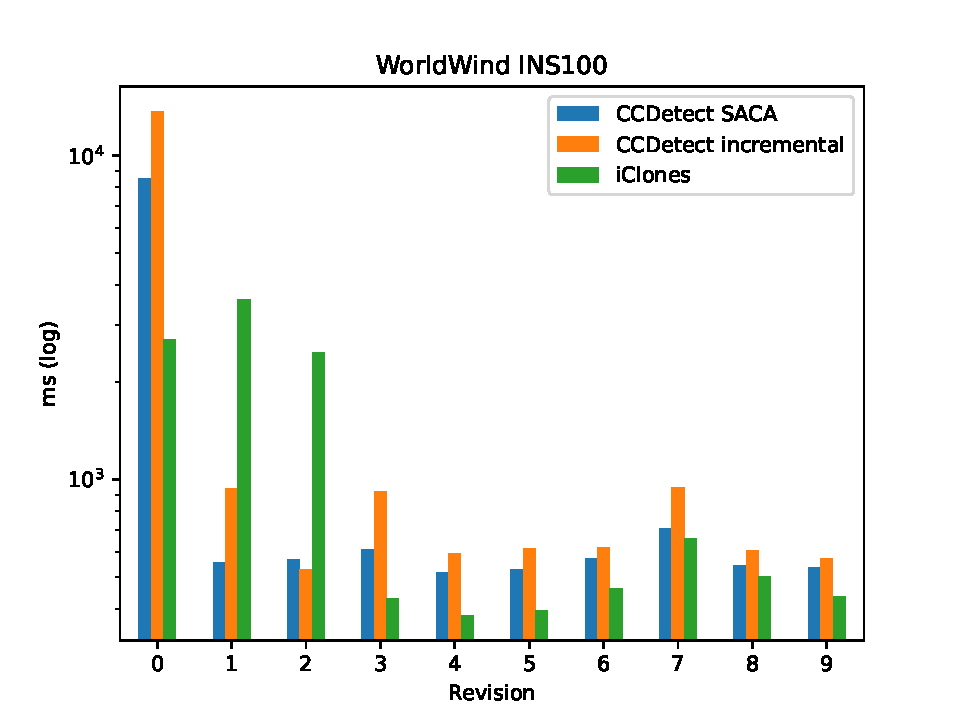
\includegraphics[width=0.49\textwidth]{figures/performancegraphs/WorldWind_INS100.pdf}
    \end{center}
    \caption{WorldWind performance benchmark}
    \label{fig:WorldWind}
\end{figure}

\vfill

\newpage
\null
\vfill

\begin{figure}[H]
    \begin{center}
        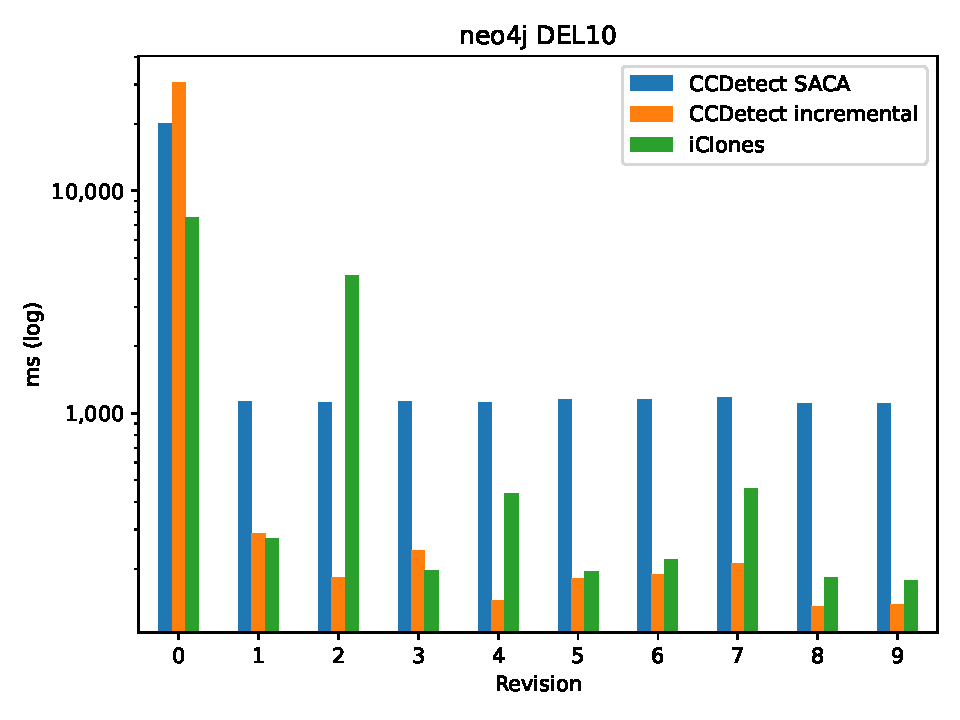
\includegraphics[width=0.49\textwidth]{figures/performancegraphs/neo4j_DEL10.pdf}
        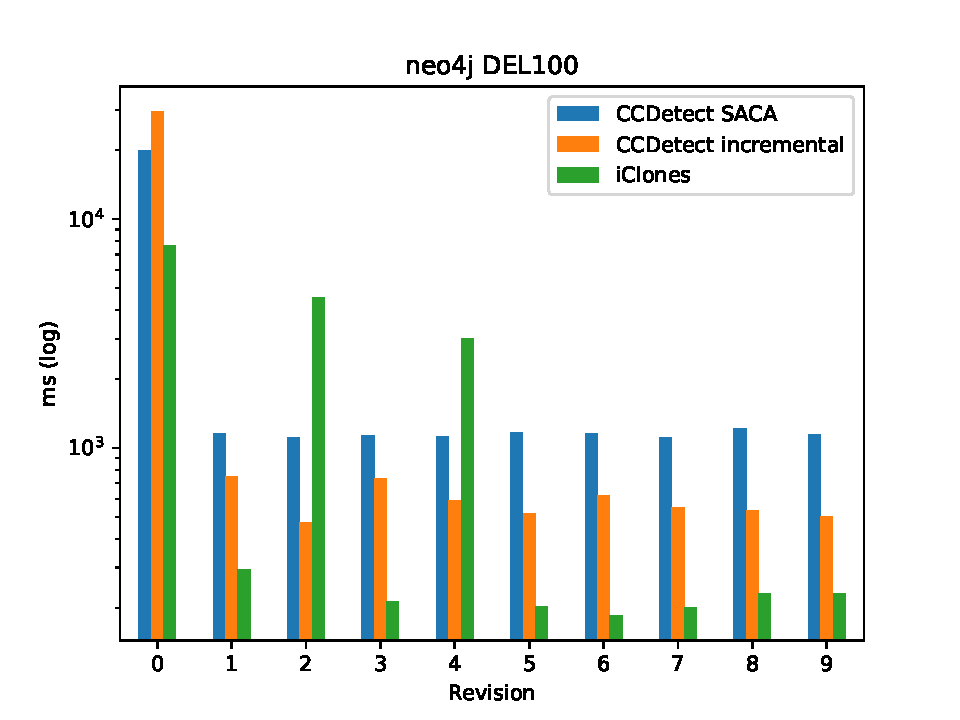
\includegraphics[width=0.49\textwidth]{figures/performancegraphs/neo4j_DEL100.pdf}
        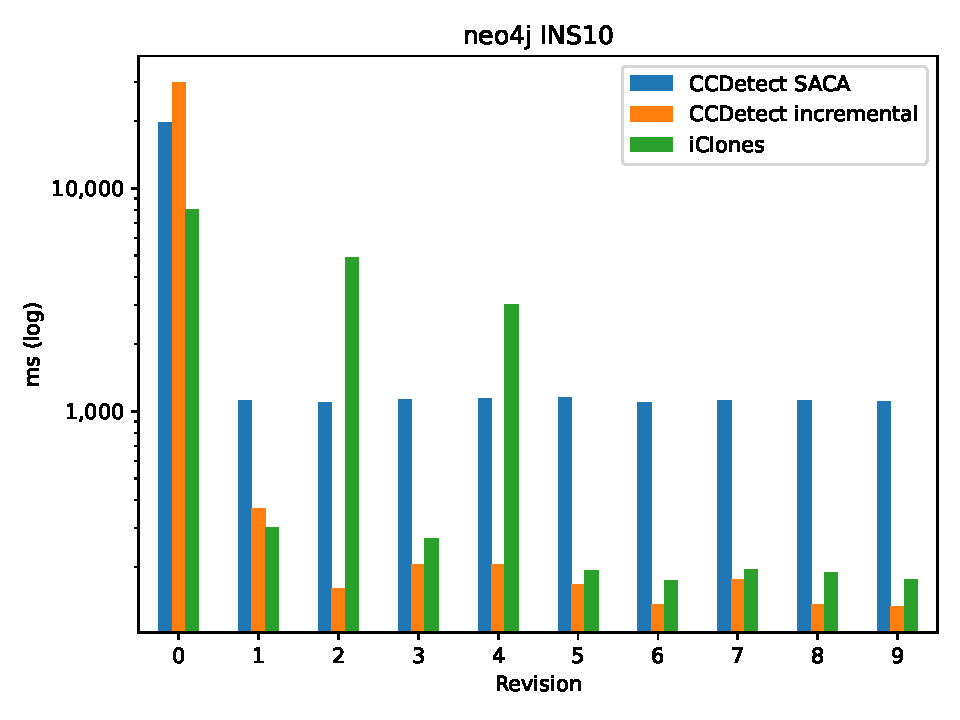
\includegraphics[width=0.49\textwidth]{figures/performancegraphs/neo4j_INS10.pdf}
        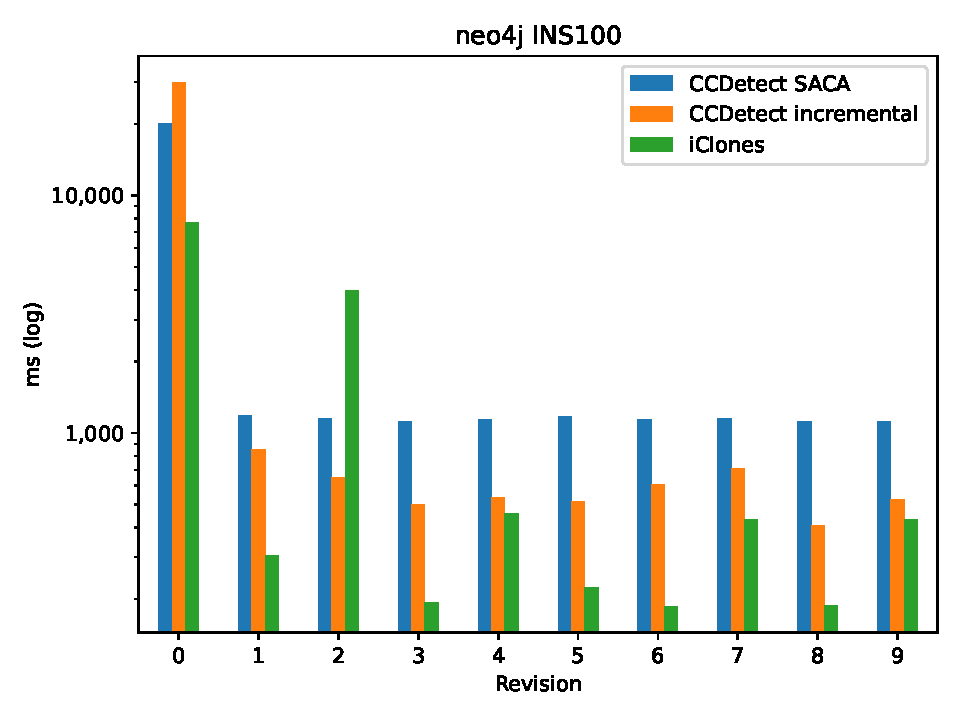
\includegraphics[width=0.49\textwidth]{figures/performancegraphs/neo4j_INS100.pdf}
    \end{center}
    \caption{neo4j performance benchmark}
    \label{fig:neo4j}
\end{figure}

\vfill

\newpage
\null
\vfill

\begin{figure}[H]
    \begin{center}
        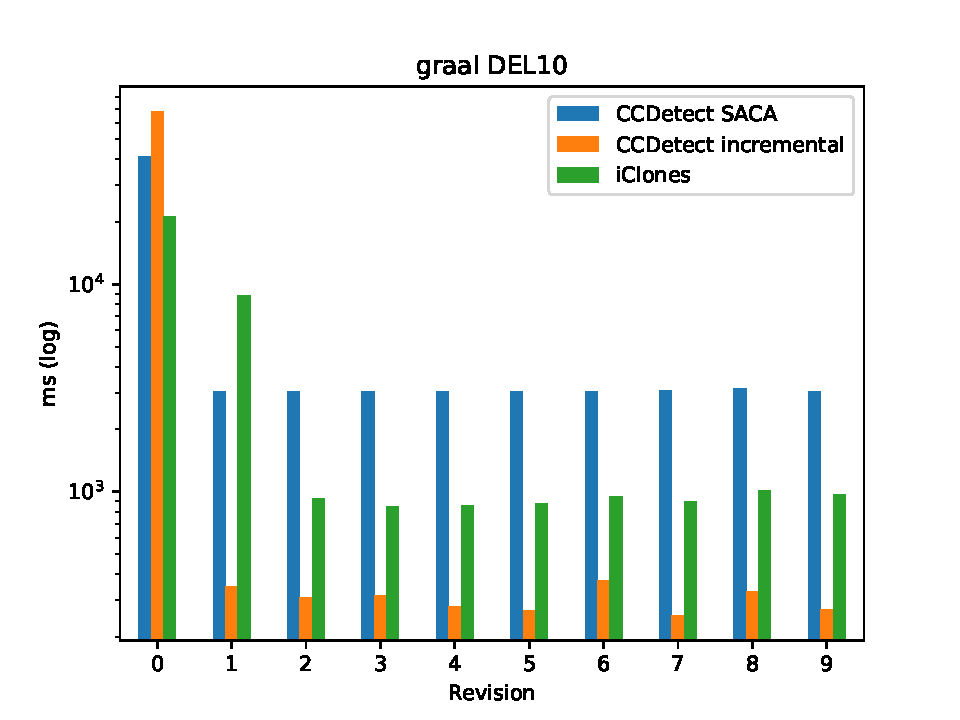
\includegraphics[width=0.49\textwidth]{figures/performancegraphs/graal_DEL10.pdf}
        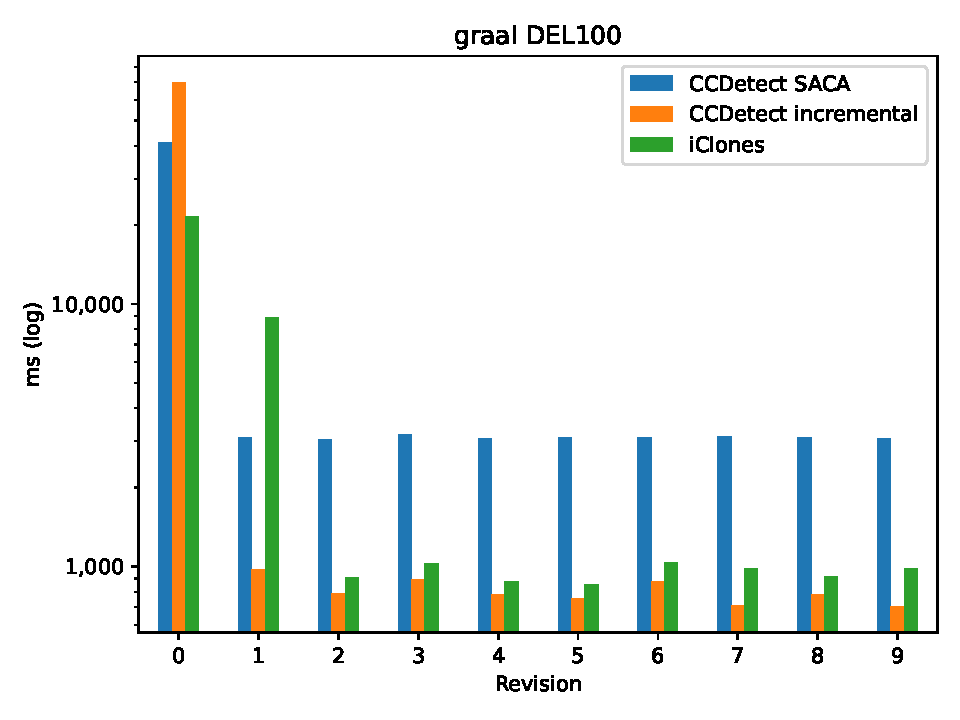
\includegraphics[width=0.49\textwidth]{figures/performancegraphs/graal_DEL100.pdf}
        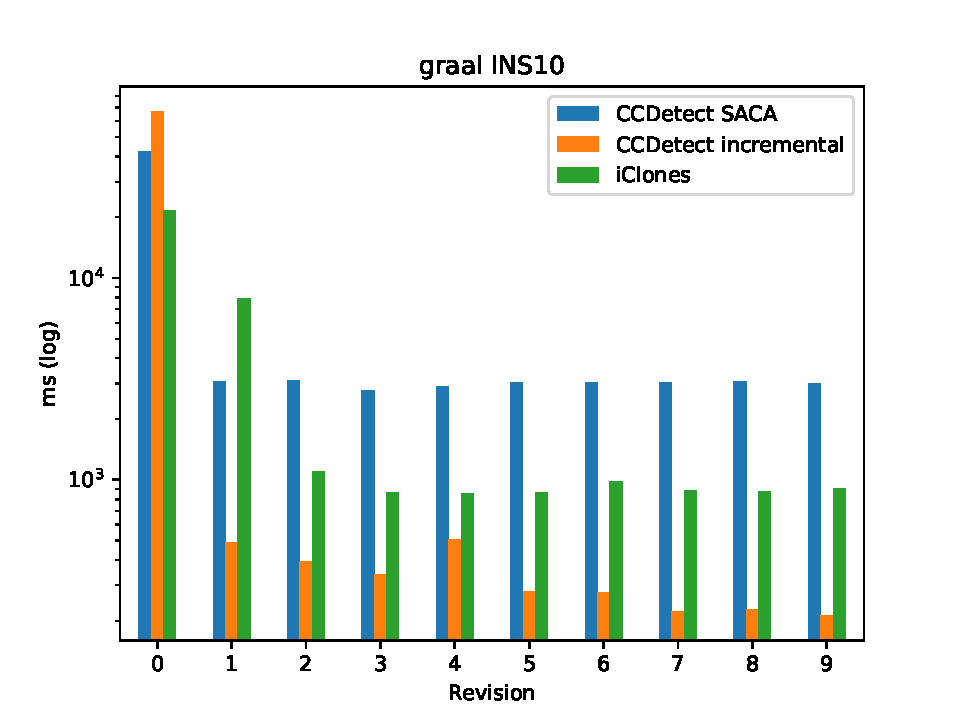
\includegraphics[width=0.49\textwidth]{figures/performancegraphs/graal_INS10.pdf}
        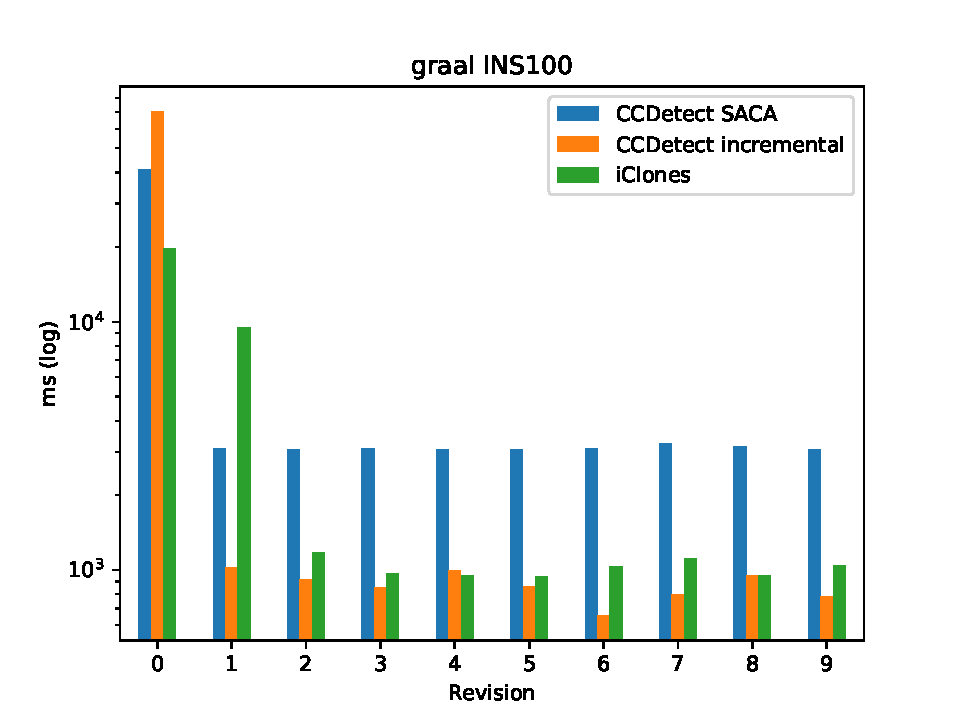
\includegraphics[width=0.49\textwidth]{figures/performancegraphs/graal_INS100.pdf}
    \end{center}
    \caption{graal performance benchmark}
    \label{fig:graal}
\end{figure}

\vfill

\newpage
\null
\vfill

\begin{figure}[H]
    \begin{center}
        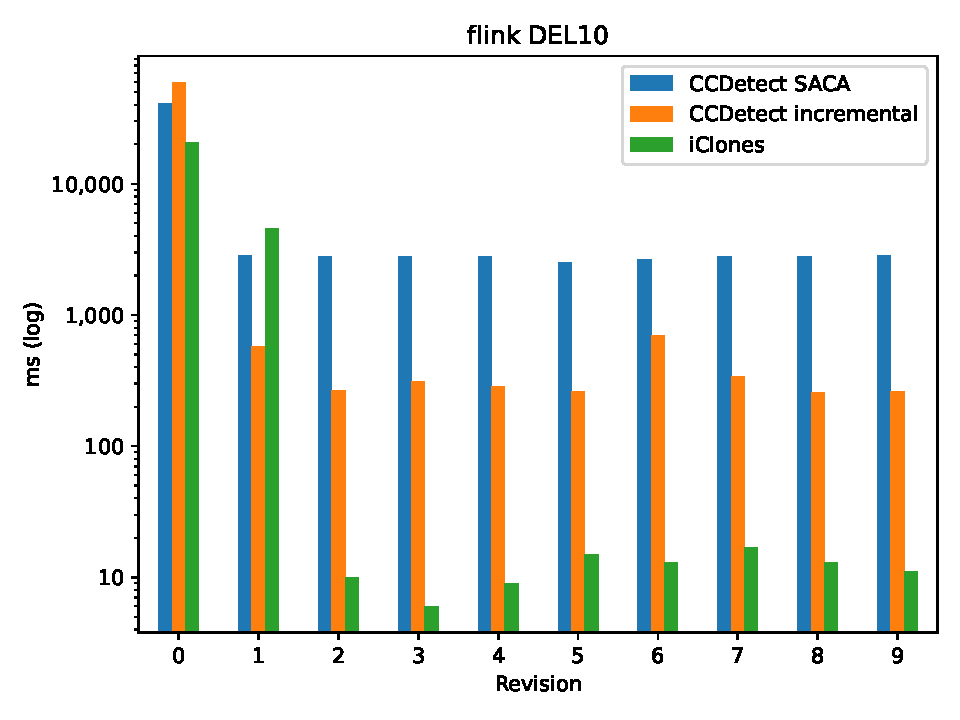
\includegraphics[width=0.49\textwidth]{figures/performancegraphs/flink_DEL10.pdf}
        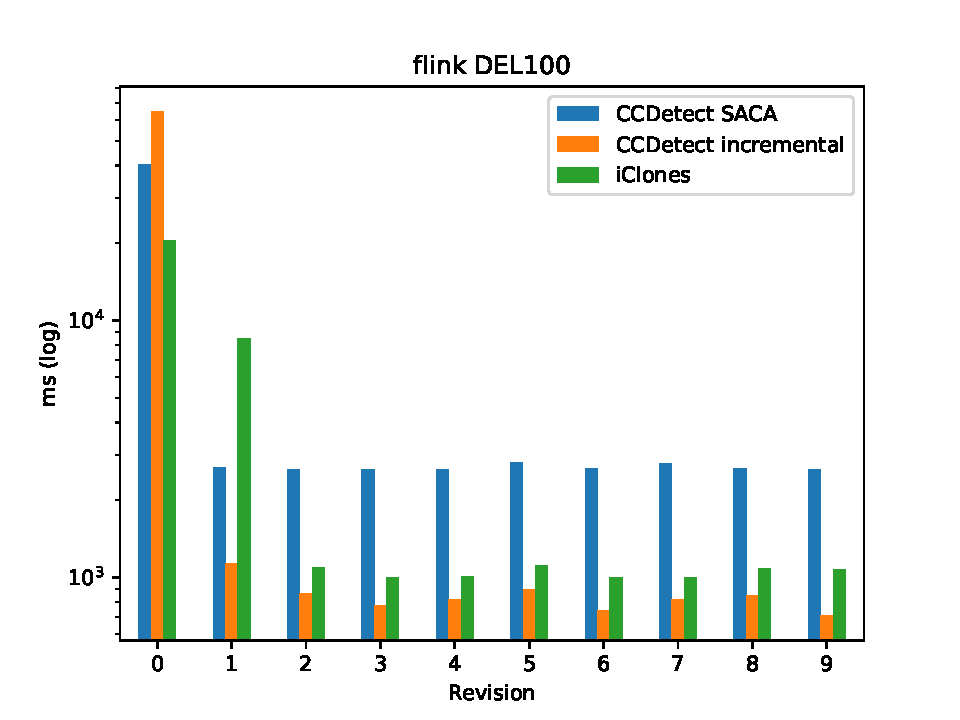
\includegraphics[width=0.49\textwidth]{figures/performancegraphs/flink_DEL100.pdf}
        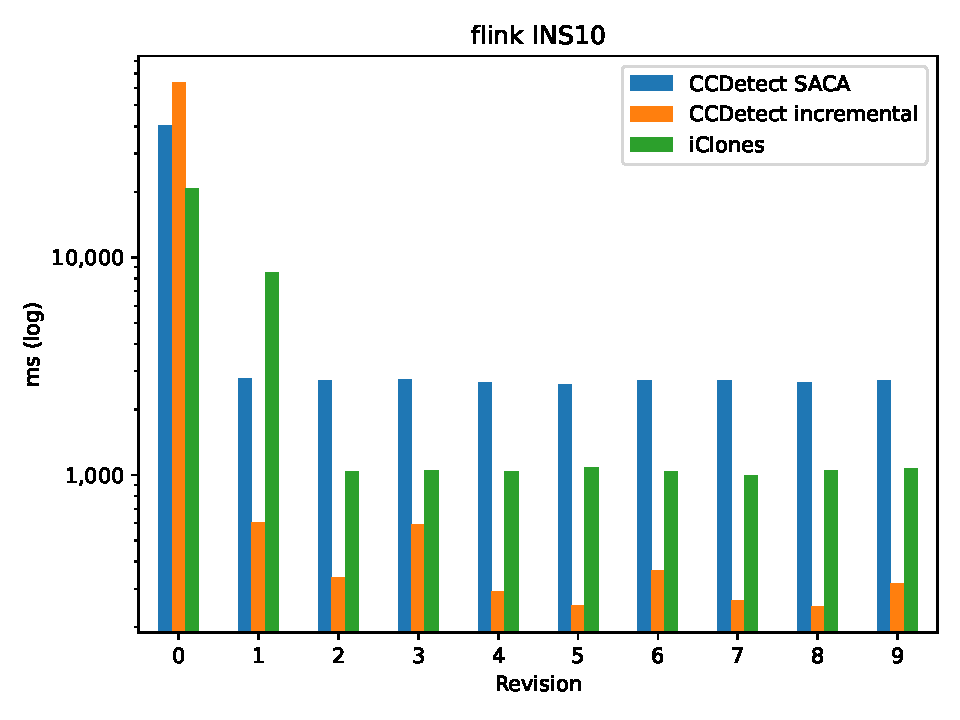
\includegraphics[width=0.49\textwidth]{figures/performancegraphs/flink_INS10.pdf}
        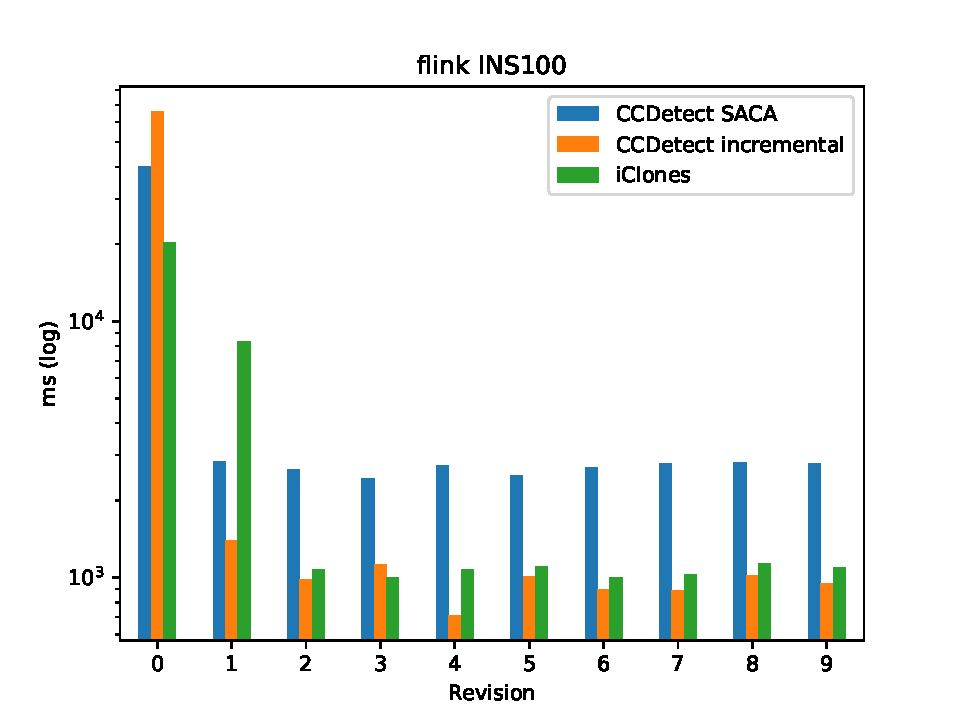
\includegraphics[width=0.49\textwidth]{figures/performancegraphs/flink_INS100.pdf}
    \end{center}
    \caption{flink performance benchmark}
    \label{fig:flink}
\end{figure}

\vfill

\newpage
\null
\vfill
\begin{figure}[H]
    \begin{center}
        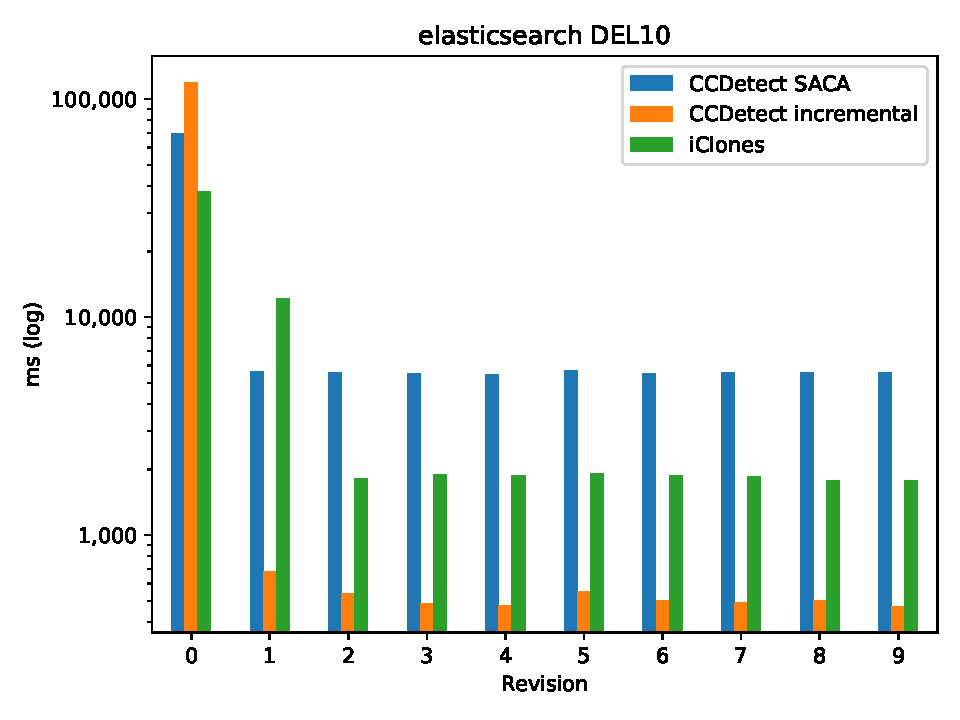
\includegraphics[width=0.49\textwidth]{figures/performancegraphs/elasticsearch_DEL10.pdf}
        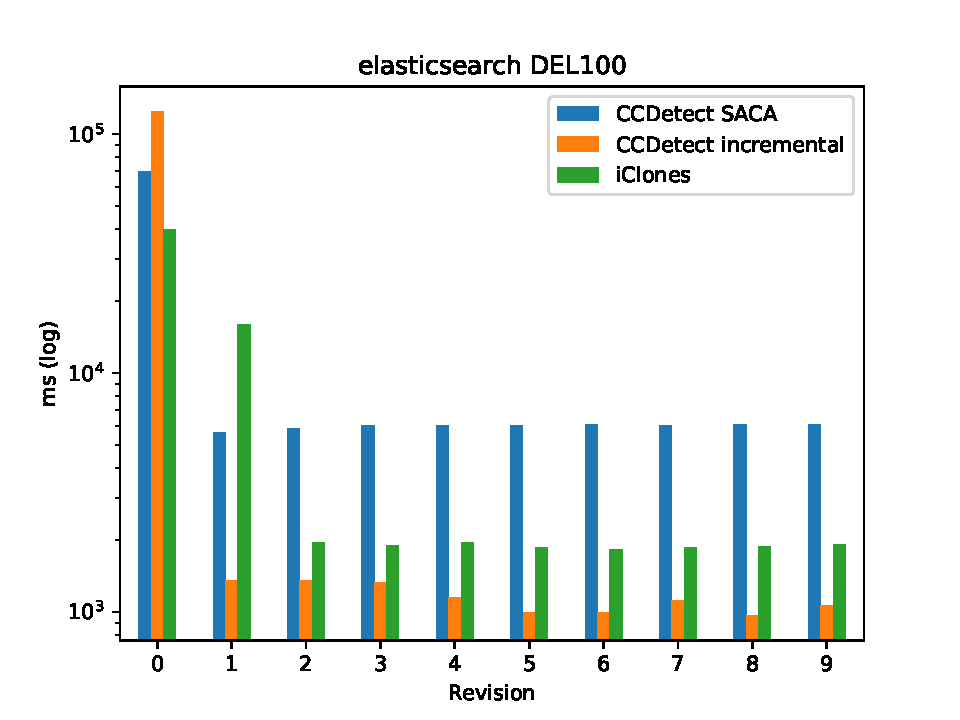
\includegraphics[width=0.49\textwidth]{figures/performancegraphs/elasticsearch_DEL100.pdf}
        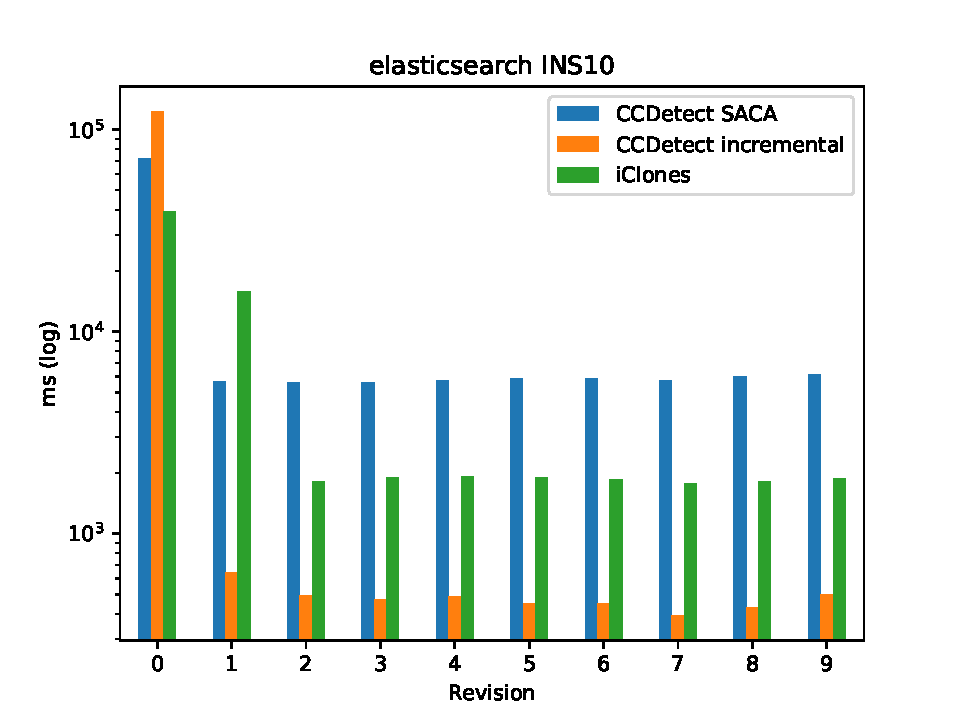
\includegraphics[width=0.49\textwidth]{figures/performancegraphs/elasticsearch_INS10.pdf} 
        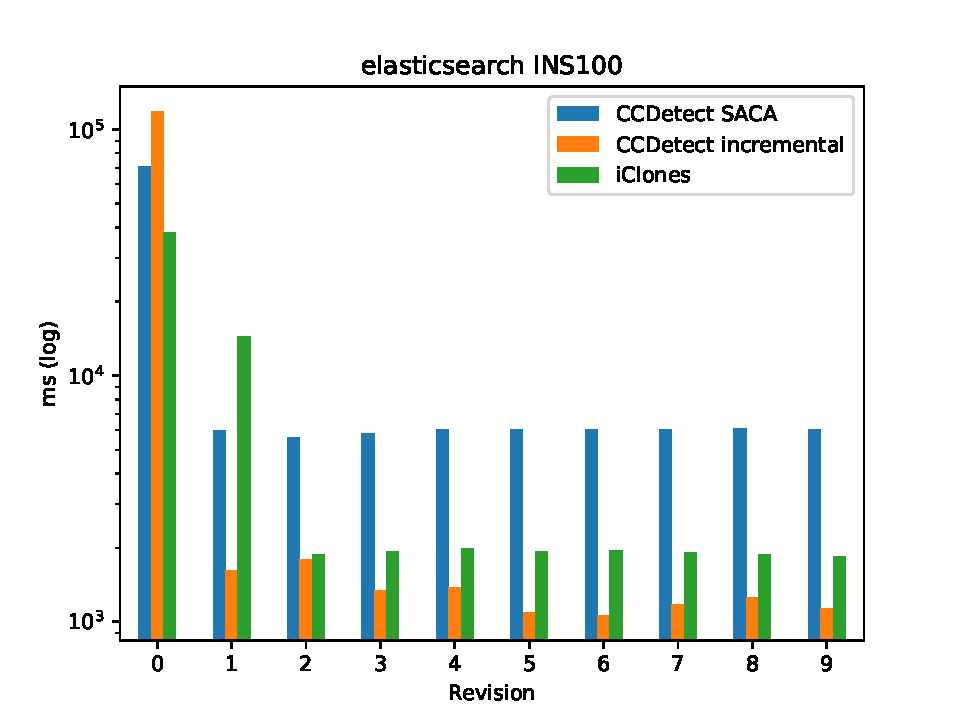
\includegraphics[width=0.49\textwidth]{figures/performancegraphs/elasticsearch_INS100.pdf} \end{center}
    \caption{elasticsearch performance benchmark}
    \label{fig:elasticsearch}
\end{figure}

\vfill

\newpage
\null
\vfill

\begin{figure}[H]
    \begin{center}
        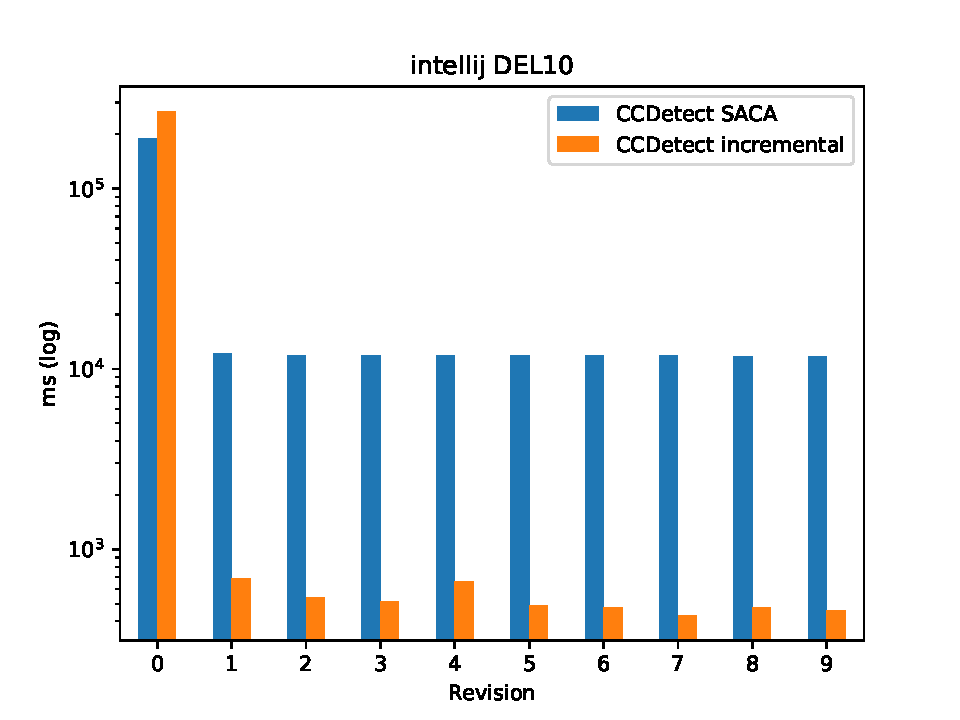
\includegraphics[width=0.49\textwidth]{figures/performancegraphs/intellij_DEL10.pdf}
        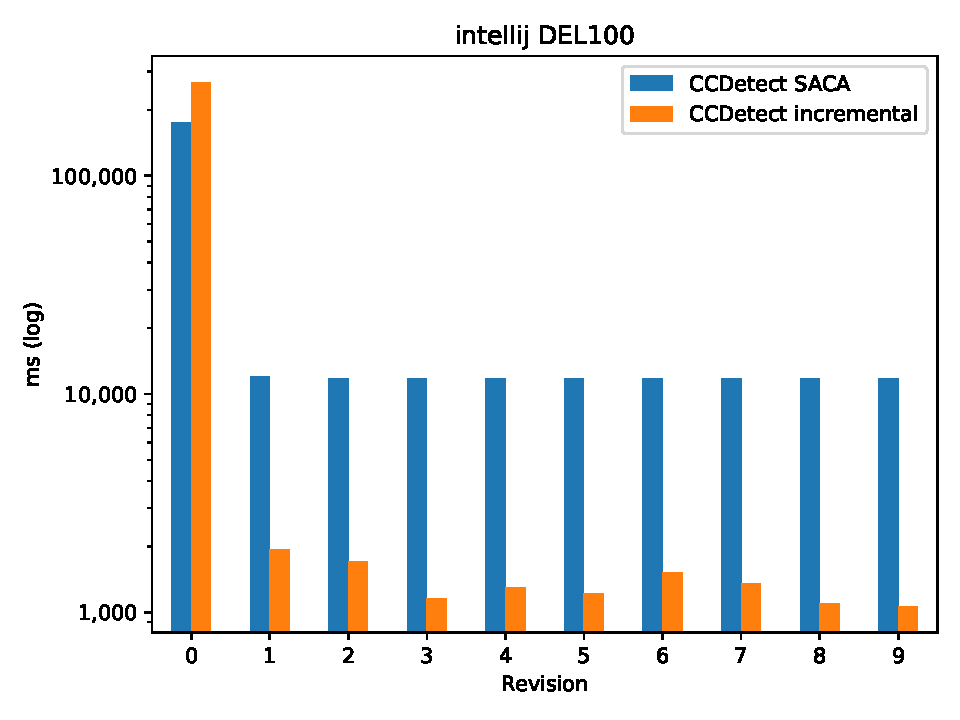
\includegraphics[width=0.49\textwidth]{figures/performancegraphs/intellij_DEL100.pdf}
        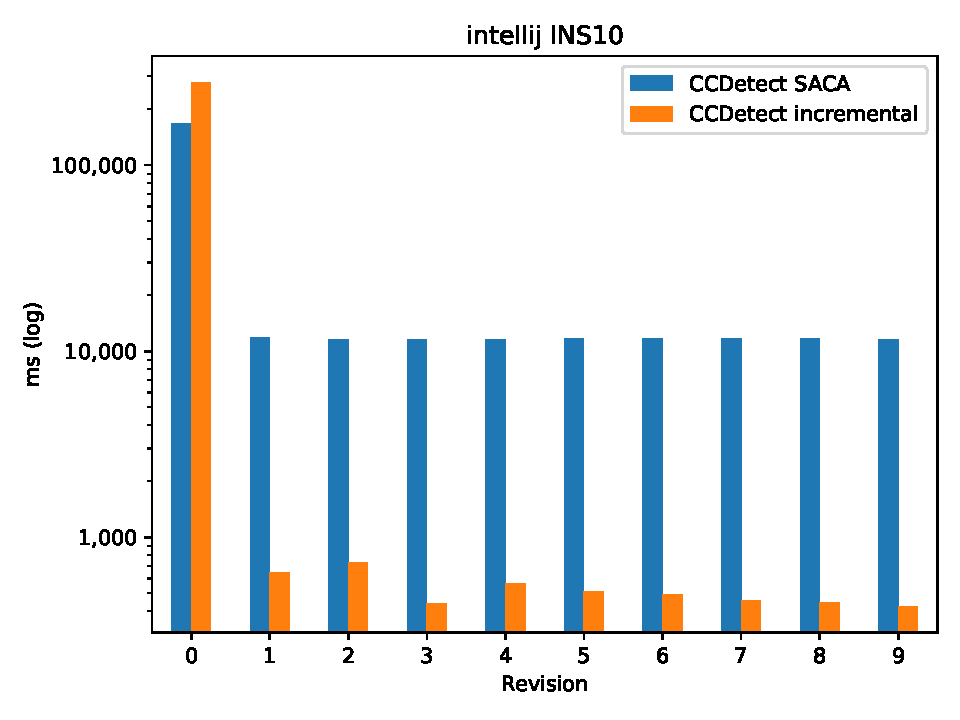
\includegraphics[width=0.49\textwidth]{figures/performancegraphs/intellij_INS10.pdf}
        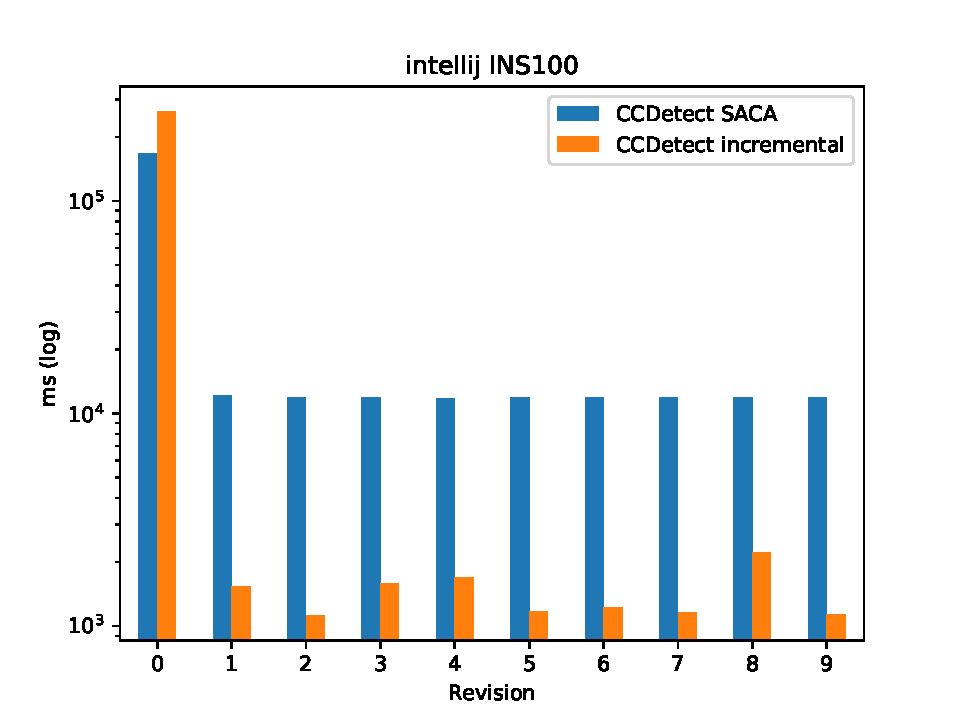
\includegraphics[width=0.49\textwidth]{figures/performancegraphs/intellij_INS100.pdf}
    \end{center}
    \caption{intellij-community performance benchmark}
    \label{fig:intellij}
\end{figure}

\vfill

\newpage
\null
\vfill

\begin{figure}[H]
    \begin{center}
        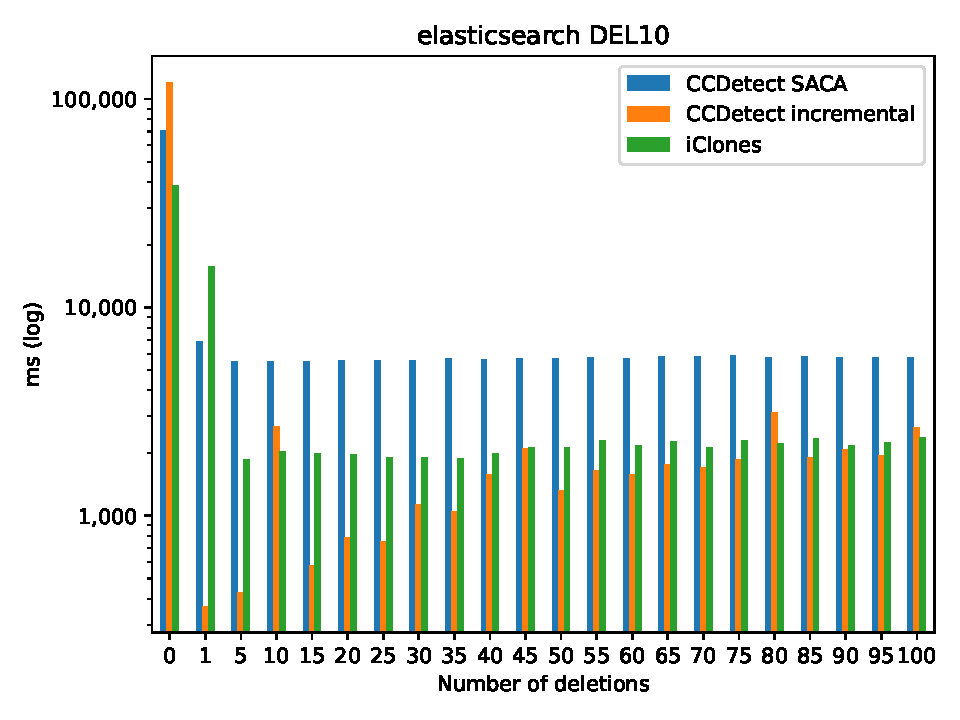
\includegraphics[width=0.49\textwidth]{figures/incedit_performancegraphs/elasticsearch_DEL10.pdf}
        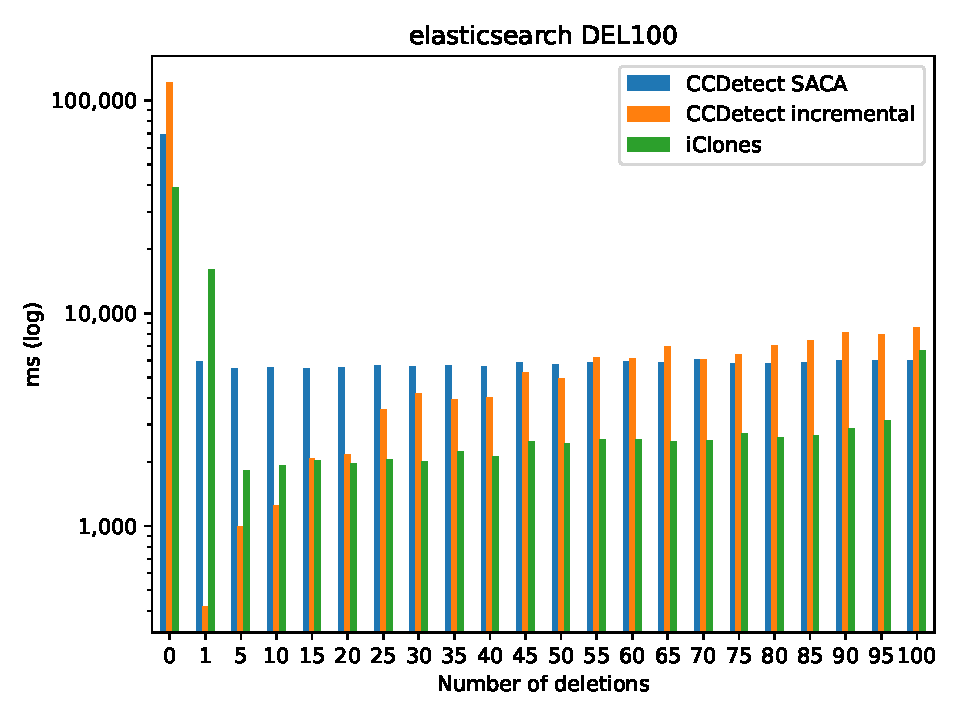
\includegraphics[width=0.49\textwidth]{figures/incedit_performancegraphs/elasticsearch_DEL100.pdf}
        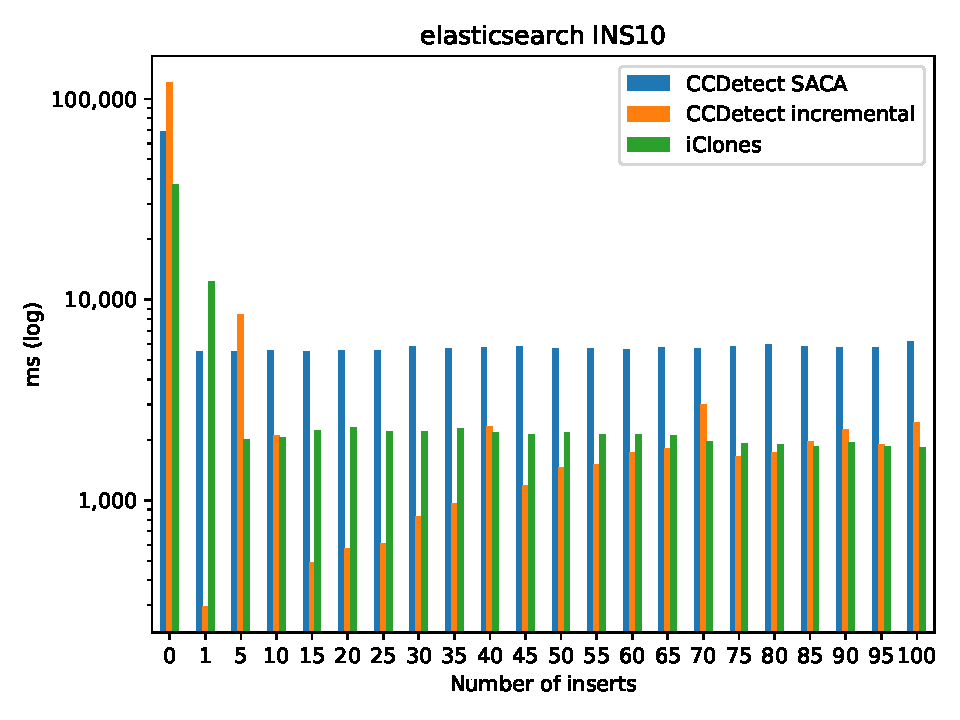
\includegraphics[width=0.49\textwidth]{figures/incedit_performancegraphs/elasticsearch_INS10.pdf}
        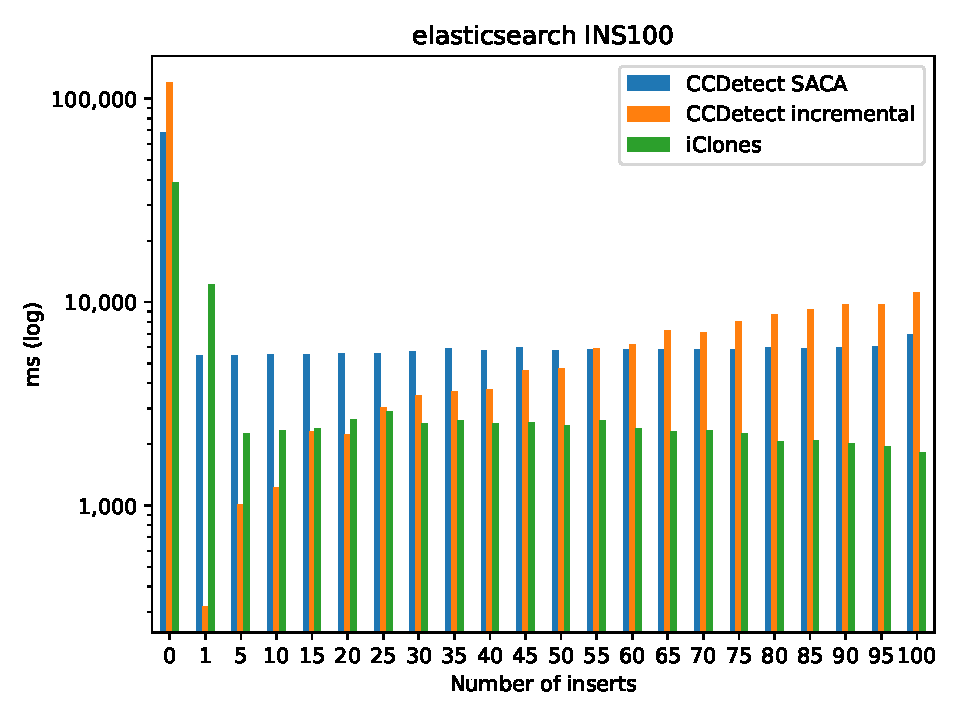
\includegraphics[width=0.49\textwidth]{figures/incedit_performancegraphs/elasticsearch_INS100.pdf}
    \end{center}
    \caption{Elasticsearch performance benchmark with increasing number of edits}
    \label{fig:elasticsearch_inc}
\end{figure}

\vfill
\newpage

\section{Memory usage}

Another important aspect of clone detection tools and especially IDE tools, is the memory
usage of the tool. As CCDetect-LSP is primarily implemented as an IDE tool, it is
important that the tool can run alongside other IDE tools and applications. Therefore, we
will in this section analyze the memory usage of CCDetect-LSP and again compare the SACA
detection, incremental detection and iClones. To simplify this analysis, we will for each
code base run one of the tests we previously ran for the performance benchmark, and
observe the peak memory usage of each algorithm, using the JProfiler\footnote{JProfiler:
https://www.ej-technologies.com/products/jprofiler/overview.html} profiling tool. In our
experience, the clone detection tools we are evaluating in this scenario does not have
large spikes in memory usage, and generally stabilizes around the peak memory usage.
Therefore, we only observed the peak memory usage, as it seems to represent the amount of
memory which would be required to run each tool in an IDE scenario.

JProfiler provides a live memory profiling overview which records the memory usage of a
running JVM process every $2$ seconds. Figure \ref{fig:memoryusage} shows the results of
the memory usage test. iClones is again left out for the intellij code base, as the memory
usage exceeded 16GB.       

\begin{figure}[t]
    \begin{center}
        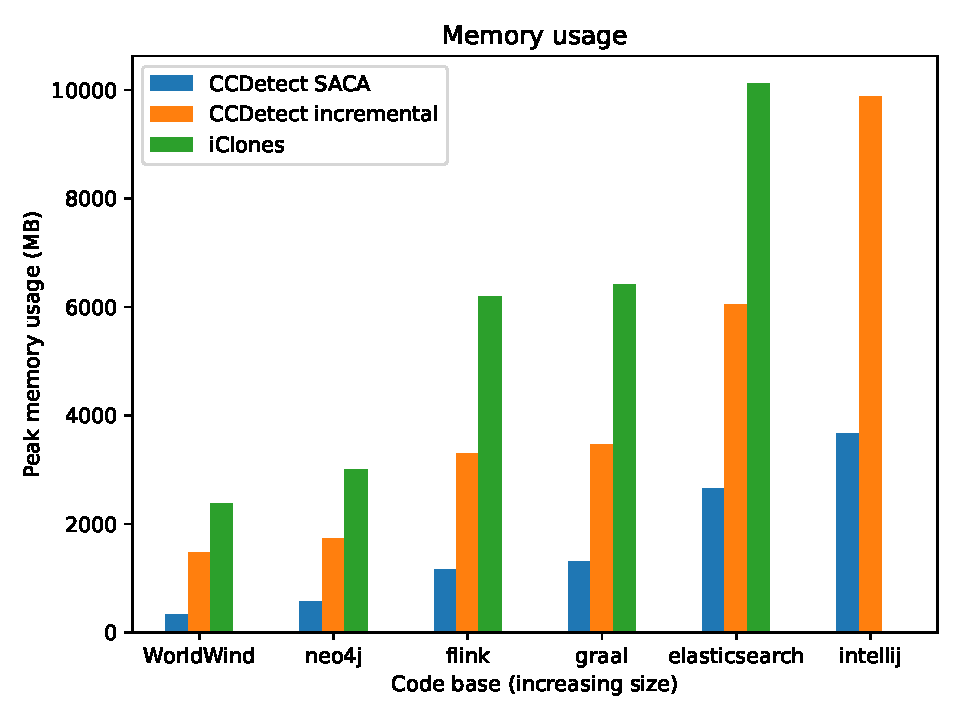
\includegraphics[width=0.95\textwidth]{figures/memoryusage.pdf}
    \end{center}
    \caption{Memory usage of each tool when running the DEL10 test for each code base.}
    \label{fig:memoryusage}
\end{figure}

\section{Languages and IDEs}

CCDetect-LSP attempts to achieve the goals of being IDE agnostic by utilizing LSP, and
programming language agnostic by utilizing Tree-sitter. In this section we will quickly go
over our experience with using these tools, and what we have implemented and tested to
determine if these goals are met.

\subsection*{Language agnostic}

For the goal of being language agnostic, we have tried CCDetect-LSP with multiple
languages, including Java, Python, C, Rust, JavaScript, and Go. To add a new language to
CCDetect-LSP all that is needed to be done is to download the correct grammar into the
\verb|grammars/| directory of the CCDetect-LSP source code, and add one case to a
match-statement in order for CCDetect-LSP to tie that grammar to a certain file-type. From
there, the client needs to change its configuration to the new language. This involves
only changing two configuration parameters, the file-type to analyze, and the Tree-sitter
query to be used in the fragment selection phase. Determining the Tree-sitter query may
not be trivial in some languages, but we suspect that the most common choices would be
either selecting the root node of the AST, or all methods or
functions\footnote{Tree-sitter queries for multiple languages are shown in the README file
of the CCDetect-LSP source code.}. If type-2 detection should be enabled, the client needs
to provide a list of token types which should be normalized for that language.

Initial experiments show that CCDetect-LSP seems to work flawlessly on most languages.
These experiments are not shown in the thesis and are based purely on our experience with
testing the tool on different code bases. While we cannot objectively tell if all clones
are detected without having an oracle like the BigCloneBench for each code base, the
experience of browsing and navigating clones seems to work as well when switching between
different languages. For example, we explored the source code of both the Rust and Go
compilers in their respective languages, and we were able to locate thousands of clones in
each code base (token threshold 100).

While our testing of multiple languages was not extensive, only one language we tested did
not work flawlessly out of the box. The Tree-sitter grammar for C had a weird quirk where
not every token had its own leaf-node in the AST. For example, the string literal token
did not have a distinct leaf-node for the string value. Therefore, functions which had
completely different string literals in them could be considered clones. This resulted in
some clones being detected which were not clones at all. Even if this issue was
preventable by treating some AST nodes differently, we consider this to be an instance
where CCDetect-LSP did not have perfect language support.

\subsection*{IDE agnostic}

CCDetect-LSP can communicate with any IDE which can act as an LSP client. We have tested
CCDetect-LSP on two IDEs which have great LSP support, Neovim\footnote{Neovim:
\url{https://neovim.io/}} and VSCode\footnote{VSCode:
\url{https://code.visualstudio.com/}}. 

For Neovim, only a configuration file needs to be setup, where we specify the command
which launches the LSP server, which file-type the LSP server should be launched on, and
the rest of the configuration which CCDetect-LSP needs. Diagnostics and code-actions work
out of the box, but a diagnostic view which shows all code clones requires an extra plugin
such as Telescope\footnote{Telescope:
\url{https://github.com/nvim-telescope/telescope.nvim}}. Neovim does not support the
\verb|DiagnosticRelatedInformation| information which can be attached to diagnostics,
therefore listing matches and navigating to them is achieved with code-actions.

For VSCode, a small extension (plugin) had to be created, which simply uses the built-in
APIs of VSCode to launch the LSP server on the correct file-type with the correct
configuration options. Once launched, VSCode has full LSP support, including diagnostics
with match information, code-actions and a nice diagnostic view which displays all code
clones. VSCode running this extension was shown in figure \ref{fig:vscodeclones} in
\cref{lspimplementation}. While the configuration settings such as token threshold and
language is currently hard-coded into the extension, we imagine it would be simple to
create a GUI configurator for CCDetect-LSP in VSCode. It could also be possible to use the
\verb|didChangeConfiguration| message defined by LSP to change the configuration as the
LSP server is running, which would allow changing for example the clone token threshold
without restarting the LSP server. 
